\documentclass[10pt,a4paper]{article}
\usepackage[justification=centering]{caption}
%%%%%%%%%%%%%%%%%%%%%%%%%%%
% MODIFY:

\newcommand{\authorA}{ALEX PASQUALI 
% (03754113)
}
\newcommand{\authorB}{NICOLA GUGOLE 
% (03753996)
}
\newcommand{\groupNumber}{A} % - YOUR GROUP NUMBER
\newcommand{\exerciseNumber}{4} % - THE NUMBER OF THE EXERCISE
\newcommand{\sourceCodeLink}{https://github.com/AlexPasqua/MLCMS-project}

\newcommand{\workPerAuthor}{
\authorA&Task 1&50\%\\
      &Task 2&50\%\\
      &Task 3&50\%\\
      &Task 4&50\%\\
      &Task 5&50\%\\
      \hline
\authorB&Task 1&50\%\\
      &Task 2&50\%\\
      &Task 3&50\%\\
      &Task 4&50\%\\
      &Task 5&50\%\\
}

%%%%%%%%%%%%%%%%%%%%%%%%%%%

%%
% imports for the exercise sheets
%

\usepackage[utf8]{inputenc}
\usepackage{amsmath}
\usepackage{amsfonts}
\usepackage{amssymb}

\usepackage[yyyymmdd]{datetime}
\renewcommand{\dateseparator}{--}

\usepackage[left=2cm,right=2cm,top=3cm,bottom=3cm]{geometry}

\usepackage{hyperref}

\usepackage{amsthm}
\newtheorem{lem}{Lemma}
\newtheorem{thm}{Theorem}
\newtheorem{cor}{Corollary}
\newtheorem{rem}{Remark}
\newtheorem{definition}{Definition}
\newtheorem{ter}{Terminology}

\usepackage{graphicx}

\newcommand{\M}{\mathcal{M}}
\newcommand{\N}{\mathcal{N}}
\newcommand{\K}{\mathcal{K}}
\newcommand{\SPDk}{\mathbb{P}^k}
\newcommand{\vol}{\text{vol}}

\newcommand{\Figref}[1]{Figure~\ref{#1}}
\newcommand{\figref}[1]{figure~\ref{#1}}
\newcommand{\Eqnref}[1]{Equation~(\eqref{#1})}
\newcommand{\eqnref}[1]{equation~(\eqref{#1})}

\usepackage{float}
\usepackage{tabularx}

\usepackage{fancyhdr}
\pagestyle{fancy}

\usepackage{totcount}
\newtotcounter{taskCounter}
\newtotcounter{pointCounter}
\newenvironment{task}[1]{\noindent\stepcounter{taskCounter}\textbf{Report on task #1}\smallbreak\hrule\smallbreak}{\smallbreak\hrule\bigbreak}


\title{Report for exercise \exerciseNumber~from group~\groupNumber}

\makeatletter
\let\thetitle\@title
\let\theauthor\@author
\let\thedate\@date
\makeatother

\providecommand{\versiondate}{\today}

\lhead{Exercise sheet \exerciseNumber}
\chead{Master Praktikum: Modelling and Simulation of Crowds WS2019/20}
\rhead{TUM}
\lfoot{Report of Group \groupNumber}
\cfoot{\thepage}
\rfoot{Last compiled: \versiondate}
\renewcommand{\headrulewidth}{0.4pt}
\renewcommand{\footrulewidth}{0.4pt}

\newcommand{\frontpage}{
\begin{center}
\textbf{\thetitle}\\~\\
\end{center}
\begin{table}[H]
\begin{tabular}{ll}
Tasks addressed:&\total{taskCounter}\\
Authors:&\authorA\\
&\authorB\\
&\authorC\\
Last compiled:&\versiondate\\
Source code:&\sourceCodeLink
\end{tabular}
\end{table}
\vfill
The work on tasks was divided in the following way:
\begin{table}[H]
\begin{tabularx}{\textwidth}{X|p{2cm}|p{2cm}}
\workPerAuthor
\end{tabularx}
\end{table}
\newpage
}

\begin{document}

\frontpage

\begin{task}{1, Summing up the paper} \label{sec:intro}
\paragraph{Introduction}
The behavior of pedestrians changes depending also on the geometry of the facility they are in, therefore it is difficult to accurately predict their movements using simple models with few parameters that do not take into account such geometry.
Neural networks (NNs) are a class of models with many adaptive parameters that do not have a fixed and direct physical meaning, for this reason they are very flexible and might be a suitable alternative for these forecasts.
Specifically, the task is the one of estimating the speed of the pedestrians as a scalar value.
Microscopic models consider people as points with a certain size and their few physical parameters can be inferred from the fundamental diagram (FD), which puts in relation the speed and the surrounding distance spacing to neighbors or obstacles.
Despite their simplicity, microscopic models can describe quite well various pedestrian flows of phenomena such as lane formation \cite{tordeux2018, helbing2005, schadschneider2009}, but the predictions in complex spatial structures remains problematic.\\
The aim of this paper is to asses whether NNs are able to accurately describe the pedestrians' behavior for various types of spatial structures.
These are compared with an FD-based model (Weidmann's Fundamental Diagram) with data gathered through experiments in a corridor/ring and bottleneck scenarios.

\paragraph{Models}
The first modelling approach is the Weidmann Fundamental Diagram, which models the speed as a continuous scalar value that is function of the mean spacing (i.e. the average distance of each pedestrian to its $K$ nearest neighbors). This is reported in Equation \ref{eq:weidmann}.

\begin{equation}\label{eq:weidmann}
    v = FD(\overline{s}_K, v_0, T, l) = v_0 \left(1 - e^{\frac{l - \overline{s}_K}{v_0 T}}\right)
\end{equation}

where $T$ is the time gap, $l$ is the pedestrian size, $v_0$ the desired speed and $s_K$ is the mean spacing, defined as $s_K = \frac{1}{K}\sum_{i=1}^K \sqrt{(x - x_i)^2 + (y - y_i)^2}$, with $(x_i,y_i)$ denoting the $i$-th nearest neighbor's position.\\

The second approach is a fully-connected feed-forward neural network.
It takes $2K+1$ inputs, namely the mean spacing $s_K$ and the $K$ relative positions $(x - x_i, y - y_i)$.

\paragraph{Data}
The data used in the paper is part of the online database of pedestrian experiments \cite{pedestrians-database}.
It is divided into two dataset (available at \cite{datasets}) obtained in laboratory conditions that represents the following scenarios:
\begin{itemize}
    \item Ring / Corridor (R):
    closed loop geometry of length 30m and width 1.8m with a pedestrians density level ranging from 0.25 to 2 $ped/m^2$, corresponding to a number of participants that goes from 15 to 230.
    The measurement area is 6m long and it is situated on a straight segment (that is why this scenario is also called ``corridor'').
    
    \item Bottleneck (B):
    this scenario can be seen as a corridor whose width suddenly reduces.
    The initial width is 1.8m, while the actual bottleneck assumes various width values, namely 0.70, 0.95, 1.20, 1.80m (this last value actually cancels the bottleneck effect because the width does not change).
    The number of pedestrians in this scenario is fixed to 150.
\end{itemize}
The speed for a given mean spacing differs in a scenario or the other, therefore the geometry is in part responsible for the behavior of pedestrians.
Figure \ref{fig:fd-curves} shows this phenomenon.

\begin{figure}[h]
    \centering
    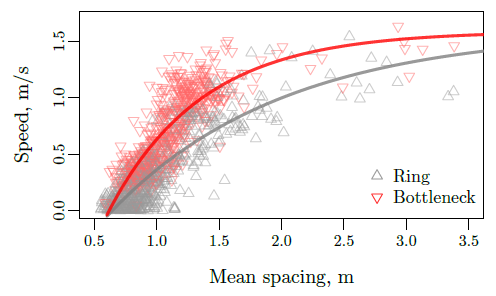
\includegraphics[scale=0.9]{images/speed_vs_mean_spacing_FD.png}
    \caption{Weidmann FD fitted on the data, showing how the speed of pedestrians differs depending also on the geometry (corridor/bottleneck).}
    \label{fig:fd-curves}
\end{figure}

\paragraph{Fitting the neural network}
The neural network is fitted on the normalized data through mean squared error $\text{MSE} = \frac{1}{N} \sum_i (v_i - \Tilde{v}_i)^2$, where $v_i$ is the actual speed and $\tilde{v}_i$ is the speed predicted by the NN.
Half of the data is kept for testing, while the rest is used for training, which is carried out using cross-validation over 50 bootstrap subsamples.
The authors do not specify the number of folds for the cross validation nor the size of the bootstrap subsamples.
In the paper, different NN architectures are tested: they are always fully-connected feed-forward NNs, but the number and the size of the hidden layers assumes the values (1), (2), (3), (4,2), (5,2) (5,3), (6,3), (10,4) and (12,5)\footnote{The number of integers in the tuples indicates the number of hidden layers and the integers themselves represent the number of neurons in the $i$-th hidden layer.}.
As shown in Figure \ref{fig:nn-training-curves}, the training error continues to decrease as the complexity of the network increases, while the testing error shows a minimum corresponding to the architecture denoted by (3), before going into overfitting.

\begin{figure}[h]
    \centering
    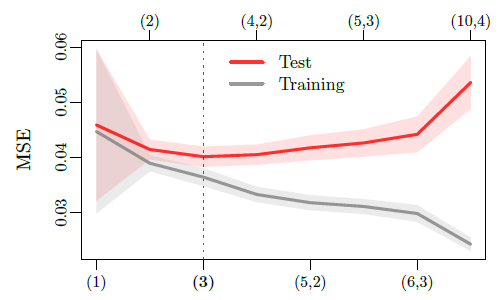
\includegraphics[scale=0.92]{images/NN_architectures_comparison_MSE.png}
    \caption{Training and testing MSE for different NN architectures.}
    \label{fig:nn-training-curves}
\end{figure}

\paragraph{Model comparison}
The Weidmann model and the NN that performed best (single hidden layer with 3 units) are compared on different combination of training/testing data.
As it is possible to observe in Figure \ref{fig:nn-vs-fd}, the NN has a lower MSE for all the these combinations, but in particular the difference is more accentuated when the models are trained with a combination of the two scenarios.
More precise numbers are reported in Table \ref{tab:nn-mes-improvement}:

\begin{table}[H]
    \centering
    \begin{tabular}{|c|c|}
        \hline
        \textbf{Training/testing scenarios} & \textbf{NN's MSE improvement}\\
        \hline
        Ring (R/R) & $\sim 5\%$\\
        Bottleneck (B/B) & $\sim 15\%$\\
        Unobserved situations (R/B, B/R) & $\sim 15\%$\\
        Training on mixed scenarios (R+B/R, R+B/B, R+B/R+B) & $\sim 20\%$\\
        \hline
    \end{tabular}
    \caption{MSE improvements of the NN over the FD model for different combination of scenarios in the training/testing data.}
    \label{tab:nn-mes-improvement}
\end{table}

\begin{figure}[h]
    \centering
    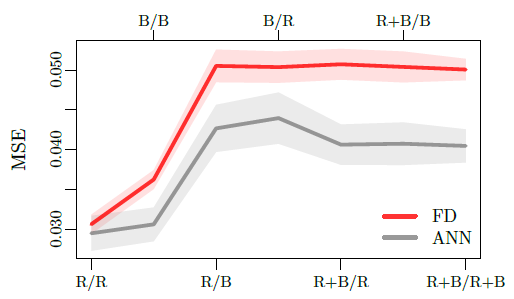
\includegraphics[scale=0.9]{images/NN_vs_FD.png}
    \caption{MSE of the FD model (in red) and the NN (in grey) with different combinations of training/testing data.
    R stands for "ring/corridor" while B represents the bottleneck.
    The letter on the left of the slash indicates the scenario(s) on which the models have been trained and the one after the slash indicates the scenario(s) used for testing.}
    \label{fig:nn-vs-fd}
\end{figure}

The same plot of Figure \ref{fig:fd-curves} is reported in Figure \ref{fig:fd-curves-fitted-nn-preds}, but the FD model has been fitted on the NN's predictions.
As it is possible to notice, the network is able to differenciate the type of geometry, even though the predictions are more mixed than the observations, where the two ``clusters" belonging to one scenario or the other are much more distinct leading to two FD curves that are more spread apart.

\begin{figure}[H]
    \centering
    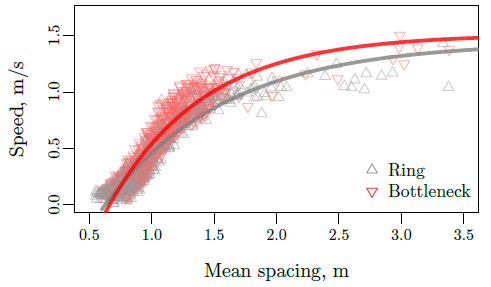
\includegraphics[scale=0.9]{images/speed_vs_mean_spacing_NN.png}
    \caption{FD model fitted on the NN's predictions.}
    \label{fig:fd-curves-fitted-nn-preds}
\end{figure}
\end{task}


\begin{task}{2, Implementation of the neural network}
Objective of this task is to discuss all the relevant aspects needed for the implementation of the models as well as their training. To reach a comparability between the implementation and the resulting paper we needed to construct and process the data following closely the paper's method. This proved to be non trivial because of the paper vagueness in defining their chosen methodologies.\\
In the following paragraphs we are going to describe how the data is preprocessed from our side, as well as how we implemented the neural network for predicting observations and finally describe how we defined the FD model through a suited neural network training. 

\paragraph{Data Preprocessing}
The data provided by the paper are taken from experiments
at bottlenecks and in corridors with closed
boundary conditions. They are not elaborated already for the final task, needing therefore some preprocessing. We are given few fields, giving per each row the \textbf{pedestrian ID}, as well as the \textbf{time} (in frames) and the \textbf{position} of the pedestrian in X, Y, Z. From these data we are asked to create the data needed by the two models, which for the training respectively require:
\begin{itemize}
    \item \texttt{mean\_spacing} as input and \texttt{speed} as output regarding the \textbf{FD model}. 1 float input, 1 float output.
    \item \texttt{mean\_spacing} and \texttt{knn\_positions} (relative) as input and \texttt{speed} as output regarding the \textbf{speed predictor model}. 2k+1 float input, 1 float output.
\end{itemize}

To achieve this result we implemented various methods in the script \texttt{create\_dataset}, which implementation is shown in \textbf{\hyperref[fig:preproc-data]{Figure \ref{fig:preproc-data}}}. 

\begin{figure}[h]
    \centering
    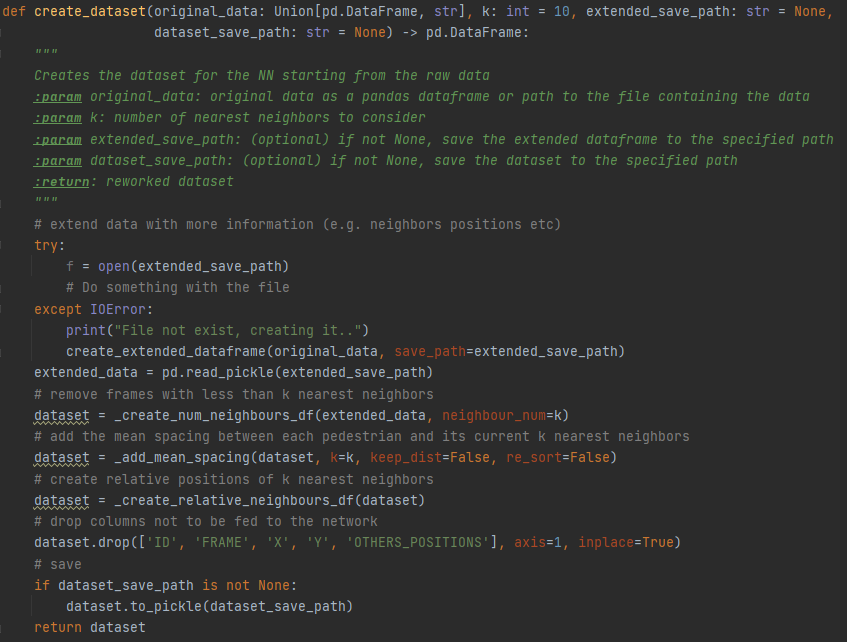
\includegraphics[scale=0.8]{images/preprocess-data.png}
    \caption{Most outer function to preprocess paper data.}
    \label{fig:preproc-data}
\end{figure}

Going through the workflow:
\begin{itemize}
    \item first of all the dataset gets \textit{extended}, if it was not already extended in the past. This means that each row (representing a certain pedestrian at a certain moment in time) is completed with ALL the neighbouring pedestrians as well as the \textbf{speed} of the pedestrian at that moment (calculated as space between two consecutive moments of that pedestrian divided by the time taken, a simple operation thanks to having frame number and frame rate). All neighbours are added to the row so that a further filtering can be done as well as to have a complete dataframe, independent from the choice of how many nearest neighbours will be considered afterwards.
    \item after creating the extended dataset (only done if necessary), all the rows with less than needed nearest neighbours are dropped.
    \item eventually the \textbf{mean\_spacing} field is created by first modifying every row such that only the \textit{k} nearest neighbour positions are maintained. When each row has the needed nearest neighbour data then the mean spacing can be easily calculated as mean of euclidean distance between each neighbour and the currently selected pedestrian.
    \item finally all nearest neighbours positions are transformed to relative nearest neighbour positions, subtracting to each neighbour the current pedestrian coordinates. At this point all data needed for training is there and all other fields (such as \textbf{frame}, \textit{pedestrian ID}, \textit{pedestrian coordinates}) are dropped.
\end{itemize}

To further simplify the data handling process we constructed the \texttt{read\_dataset} method in \texttt{utilities.py}. The method accepts a path to access the requested data and through a flag understands if the data to return has to be adequate for training the FD model or the speed predictor NN.

\paragraph{Neural Network for Speed Prediction}
Paper describes incredibly small networks, a peculiar fact when looking at the year of publishing of the paper. The networks are also not particularly complex as previously explained, being feed-forward neural networks with small hidden layers having \textit{sigmoid} as activation function and a one-node linear output layer.\\
The NN training requires \textit{bootstrapping} over many subsamples (the paper fixes the number \textbf{50}) and actuating \textit{cross validation} on the subsample. 

To basically describe how we implemented such a process we can go over the steps:
\begin{itemize}
    \item first of all we load the data needed for the NN training. We split the data into \textit{training} and \textit{testing}, following a \textbf{50/50} split as requested by the paper.
    \item secondly we start a cycle to train a model on every subsample requested by the bootstrapping technique. At the end of each model training the final losses regarding \textit{training}, \textit{validation}, and \textit{testing} are saved to have a final mean and std operation at the end of the whole bootstrapping.
    \item on each subsample the cross validation technique (we opted on a \textbf{5-fold}) is performed, which implementation is shown in \textbf{\hyperref[fig:nn-training]{Figure \ref{fig:nn-training}}}.
    \item once the k-fold cross validation is terminated the overall losses are taken as the mean over the losses of the k-folds. Also the losses std is computed. 
    \item having the results at hand allows us to select the best model, which parameters will be used to train the final model using all the training data.
\end{itemize}

\begin{figure}[h]
    \centering
    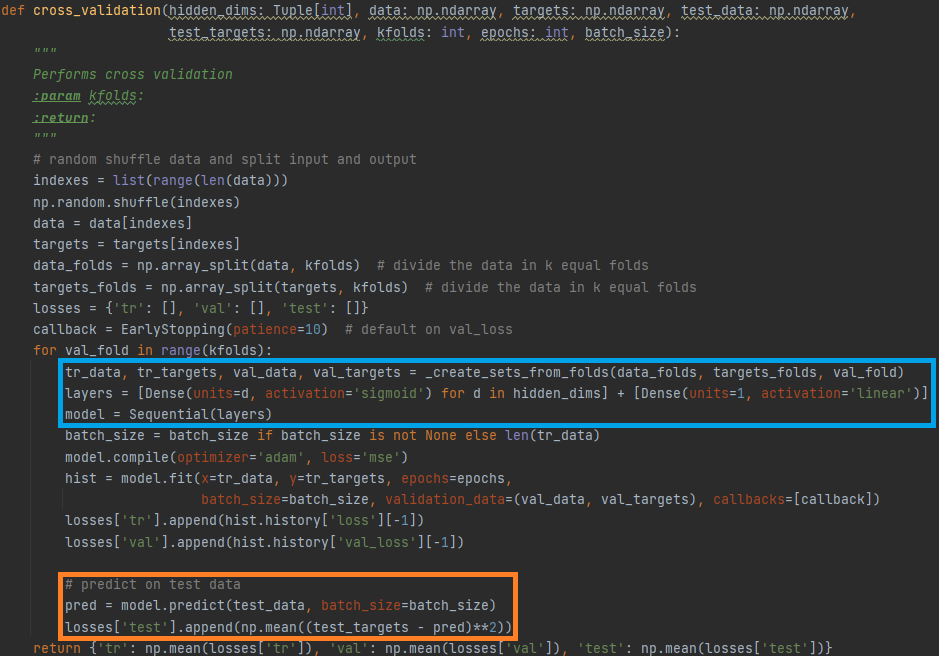
\includegraphics[scale=0.8]{images/nn_training.png}
    \caption{Cross validation per each bootstrapped subsample.}
    \label{fig:nn-training}
\end{figure}

Going more in depth at the core of the training we can discuss what is presented in \textbf{\hyperref[fig:nn-training]{Figure \ref{fig:nn-training}}}. Cross validation is performed on an initially random shuffle of the data to avoid possible correlation in consequent data of the original dataset. \textbf{Early stopping} is used as a simple yet efficient manner of getting the model to end the training as soon as it starts to overfit. The simplicity of the required models allowed us to automatically define them through a parameterized \texttt{Sequential} instantiation, as can be appreciated in the \textit{light blue} box. Finally we train the models using \textbf{MSE} as metric and \textbf{Adam} as optimizer, after testing that \textbf{SGD} resulted in a too slow training. In the end (\textit{orange} box), after fitting the model we test it on the \textit{test data} utilizing the \texttt{predict} method, to assert the model generalization capability and save the last needed loss.

\paragraph{Regression on FD model}
\textbf{\hyperref[sec:intro]{Section 1}} first introduced the model required, the \textit{Weidmann FD model}, expressed by \eqref{eq:weidmann}. The model is rather simple, composed of four parameters. We opted therefore to create a simple NN as it can allow us to model a network with all the needed output parameters for \textit{Weidmann}.\\
Since \texttt{mean\_spacing} is given in input we only need a simple NN with a single node input and a three nodes layer output. The overall implementation can be appreciated in \textbf{\hyperref[fig:fd-training]{Figure \ref{fig:fd-training}}}. For this kind of implementation we preferred \textit{model sub-classing} with respect to \textit{Sequential}, since it allows for higher modelling freedom even though it is less concise code-wise.\\
Going into details, we decided for an architecture with a single input node and a single dense hidden layer having \textit{sigmoid} as activation function (for non-linearity purpose) with three final distinct output nodes, one per each \textit{Weidmann} parameter. The output activation functions should respect the parameter domain and that is why we plugged in \textit{softplus} in all three output nodes, although one should notice how the \textit{softplus} can become a \textit{linear} for the \textit{desired speed} parameter if a more complex and bidirectional scenario is taken into consideration.\\
Eventually, looking at it from the outside, after proper training this model takes in input the \texttt{mean\_spacing} and returns exactly what presented in \eqref{eq:weidmann}, because of the formula instatiation happening in the \textit{purple} box of \textbf{\hyperref[fig:fd-training]{Figure \ref{fig:fd-training}}}.

\begin{figure}[h]
    \centering
    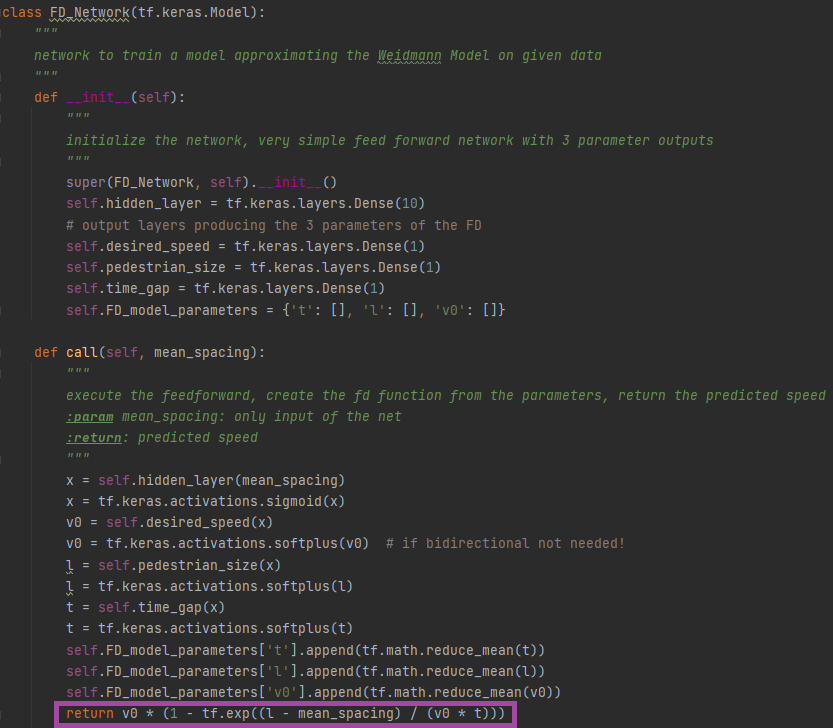
\includegraphics[scale=0.8]{images/fd_implem.png}
    \caption{Weidmann model implemented as Neural Network.}
    \label{fig:fd-training}
\end{figure}

As a final remark, we usually trained the FD network using once again \textbf{MSE} as metric and loss (between the \textit{computed} and the \textit{target speed}) with \textbf{Adam} as optimizer. Usually a small number of epochs (less than 50) was enough to reach convergence.


\end{task}


\begin{task}{3, Tests on simple examples}
A first test of validity for the implementation we constructed and described in \textbf{task 2} is done through the software \textbf{Vadere}. Constructing a self-made scenario in a closed system as this software allows for a complete control over the data generation.\\
Constructing a scenario as we need it to be is not trivial, requiring an ad hoc \textit{PostProcessor} implementation as well as some post processing of the output files themselves before having the data that can be fed to the constructed models.
\paragraph{Vadere Post Processor Implementation}
Implementing a new component in a large software such as Vadere proved to be rather complex at first, understanding which modules were needed to correctly append the new \textit{PostProcessor} into the ecosystem.

\begin{figure}[h]
    \centering
    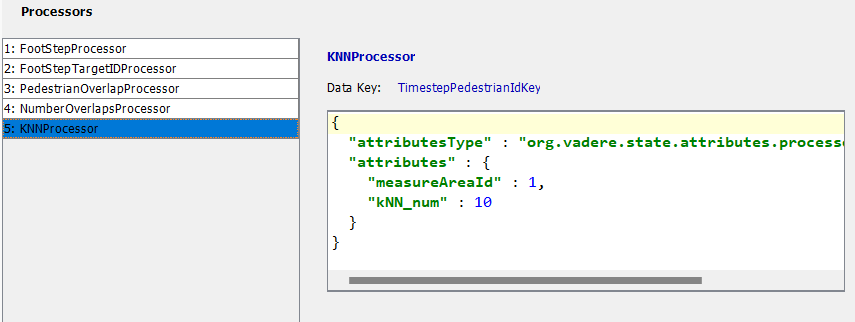
\includegraphics[scale=0.8]{images/add-proc.png}
    \caption{Adding the processor in Vadere scenario.}
    \label{fig:add-proc}
\end{figure}

Trial and errors (and many \textit{Migration errors}) led to the final implementation which is basically composed of three main classes:
\begin{itemize}
    \item \texttt{KNNAttributes}: this class is extremely basic but fundamental to the whole process. It is in fact where the main needed attributes are stored, in particular the \textit{kNN\_num} of neighbours required per each pedestrian at every possible simulation step in the output file. Another important attribute here specified is \textit{measureAreaId}, meaning the specific measurement area (there needs to be one) from where to fetch the pedestrians positions at every simulation step.
    \item \texttt{KNNPedestrianData}: a class useful to define how the single output line is composed. In particular this class contains all the needed output information, from \textit{meanSpacing} (needed both as input for the FD model as well as the NN model) to \textit{pedestrianPosition} (needed for postprocessing the speed) and finally to \textit{kNN} (a list containing all the \textit{kNN\_num} neighbours \textit{relative} positions, input of the NN model). In particular the function \texttt{toStrings} returns to the output file manager how to correctly order the information in the output file associated to \texttt{KNNProcessor}.
    \item \texttt{KNNProcessor}: the main class, updating through standard method \texttt{doUpdate} at every simulation step. When \texttt{doUpdate} is called a series of steps are performed to create the data necessary to create a new instance of \texttt{KNNPedestrianData} (new line of output):
    \begin{itemize}
        \item the measurement area is checked to get all the pedestrians inside it at the given simulation step.
        \item for each pedestrian in the measurement area a priority queue is created (to take advantage of its property of ordering).
        \item for each neighbour of a pedestrian the distance between the two is calculated as well as the relative distance. 
        \item if the priority queue (with \textit{kNN\_num} shape) is not full or the distance of the currently selected neighbour is less than the longest distance in said priority queue, then the neighbour is added.
        \item each pedestrian is checked iteratively. When for a single pedestrian all neighbours have been checked then an output line is created (\textit{timeStep}, \textit{pID}, \textit{meanSpacing}, \textit{pedestrianPosition}, \textit{kNN}), if there are enough neighbours.
    \end{itemize}
\end{itemize}

Eventually, with the implementation we propose, getting the needed data is not complex. One only has to create a scenario containing a measurement area and then navigate to \texttt{Data output} in Vadere, adding a new output file with \texttt{Data Key} equal to \texttt{TimestepPedestrianIdKey}. Then one has to add the \texttt{KNNProcessor} to the processor list and fill the needed attributes (\textbf{\hyperref[fig:add-proc]{Figure \ref{fig:add-proc}}}), which are the number of neighbours and the measurement area id. Eventually link the output file with the processor.\\
The procedure is nevertheless not complete at this point, as there is still the need for postprocessing such a ``\texttt{.txt}" file so that the input to NN model or FD model are created.

\paragraph{Post Processing of Output Files}
All the post processing can be done easily thanks to the utilities present in the file \texttt{data\_processing\_vadere.py}. The main steps are shown in \textbf{\hyperref[fig:vadere-postproc]{Figure \ref{fig:vadere-postproc}}}. First a dataframe is constructed adding the basic fields of \texttt{TIME\_STEP}, \texttt{ID} and \texttt{MEAN\_SPACING}.
The second step is taking the relative positions and porting them from the non-convenient format of ``\texttt{.txt}" to an easy to work numpy array. Eventually the only field remaining left away for execution is the \texttt{SPEED}, needed for computing the loss. Having at each row the pedestrian position and the simulation step makes the speed generation fairly easy, since what one needs is to find two following simulation steps with the same pedestrian, subtract the positions and divide by the time passed.

\begin{figure}[h]
    \centering
    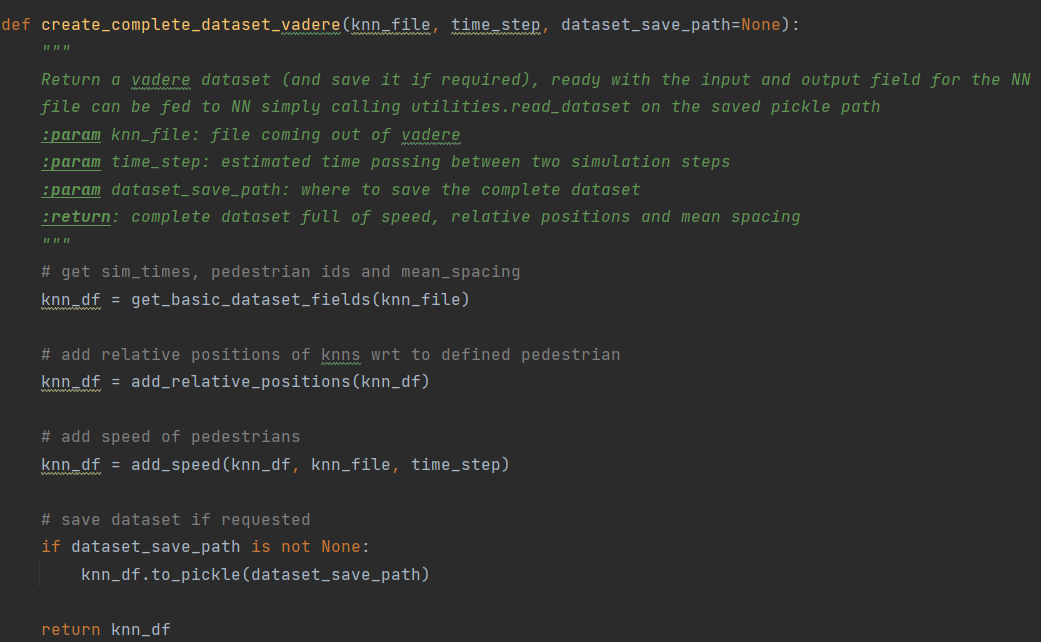
\includegraphics[scale=0.65]{images/vadere-postprocess.png}
    \caption{External function to compute all needed data for training.}
    \label{fig:vadere-postproc}
\end{figure}

The aforementioned speed generation technique seems trivial, but finding the time passed between each simulation step is not. In fact one can tell to Vadere the exact time that should pass between following steps, but the execution time as well as the algorithm for calculating trajectories (we used \textbf{OSM}) tend to not allow for such a fixed time. To get a decent approximation of said timing we created a method which goes through the ``\texttt{.traj}" file of the scenario and collects all the different times passing between simulation steps. Eventually the approximated \texttt{time\_step} is returned as the minumum of said list. We opted for the minimum instead of the mean or the max to avoid outlier effects, as well as to get the lowest possible value, which should resemble closely what the given fixed simulation parameter was.

At the end of the procedure all the unnecessary fields are dropped, leaving only the strict necessary for training and saving the result.

\paragraph{Scenarios in Details}
This paragraph has the goal of presenting the developed scenarios before showing the results.
As experiment we decided to create two different scenarios:
\begin{itemize}
    \item a \textbf{corridor} scenario (\textbf{\hyperref[fig:vadere-corridor]{Figure \ref{fig:vadere-corridor}}}), defining a corridor of 8x2 meters. The corridor describes a situation where the pedestrians (100 people) move unidirectionally (utilizing \textbf{OSM}) from source to target, getting measure in the shown area.
    
    \begin{figure}[h]
    \centering
    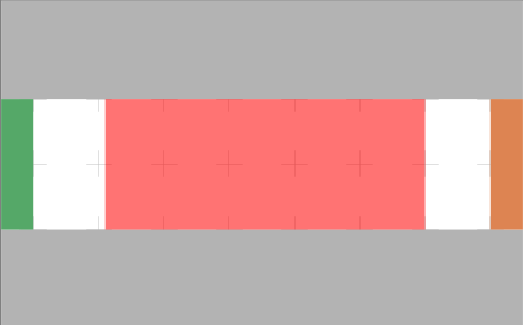
\includegraphics[scale=0.8]{images/vadere-corridor.png}
    \caption{Vadere corridor scenario.}
    \label{fig:vadere-corridor}
    \end{figure}

    \item a \textbf{bottleneck} scenario (\textbf{\hyperref[fig:vadere-bottleneck]{Figure \ref{fig:vadere-bottleneck}}}), defining a scenario 14 meters long with a 0.9 meters wide bottleneck. The bottleneck describes a situation where the pedestrians (again 100 people) move unidirectionally (utilizing \textbf{OSM}) from source to target, slowing down because of passing through the bottleneck.
    
    \begin{figure}[h]
    \centering
    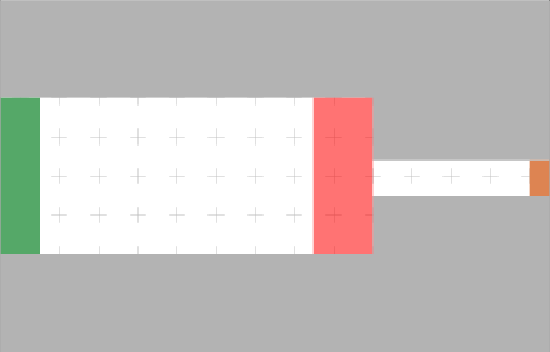
\includegraphics[scale=0.8]{images/vadere-bottleneck.png}
    \caption{Vadere bottleneck scenario.}
    \label{fig:vadere-bottleneck}
    \end{figure}
\end{itemize}

\paragraph{Results}
To validate our implementations we tested for both scenarios two different situations:
\begin{itemize}
    \item FD model trained on observations (\textit{in blue}).
    \item FD model trained on the NN's predictions (\textit{in red}), testing both the validity of FD model as well as NN's capability of representing original observations.
\end{itemize}
We tried different NN architectures, while keeping instead for the FD model the same architecture defined in \textbf{task 2}.
Moreover, since this task goes to prove the validity of the model we have not gone through validation (an important part of next task), testing the model on the training data itself. We know this is not good practice as machine learning scientists, nevertheless we once again consider this only as a validity task.\\
Starting with results coming from the \textbf{corridor} scenario, all the models we constructed utilize \textbf{Adam} as optimizer, with different architectures and training:
\begin{itemize}
    \item \textbf{FD model:} architecture as described in \textbf{task 2}.
    \item \textbf{NN model:} after different trials changing hidden layers shape and activation functions, the best performing resulted to be a model with hidden architecture \textbf{(3,3,3)} and hidden activation function \textbf{tanh}.
\end{itemize}

Results can be appreciated in \textbf{\hyperref[fig:vadere-corridor-result]{Figure \ref{fig:vadere-corridor-result}}}, where one can appreciate how the NN is capable of resembling the observations (red dots on right vs blue dots on left) and the FD model also keeps a similar behaviour in both cases.

Regarding the \textbf{MSE} values:
\begin{itemize}
    \item FD model on observations (training MSE): \textbf{0.1264}
    \item NN model predictions (training MSE): \textbf{0.0973}
    \item FD model on NN predictions (training MSE): \textbf{0.0296}
\end{itemize}

The much smaller MSE value of FD model on predictions with respect to the FD model on observations is possibly explainable by the NN's predictions, which result to be in a relatively smaller \textit{speed} range when compared to the observations.

\begin{figure}[H]
    \centering
    \subfloat[a]{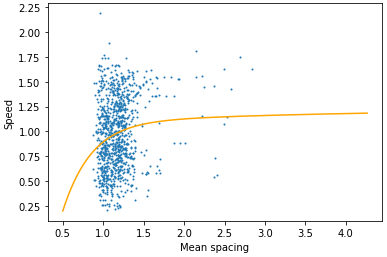
\includegraphics[scale=0.85]{images/vadere-corridor-obs.png}}
    \hfill
    \subfloat[b]{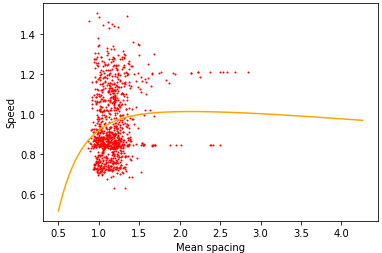
\includegraphics[scale=0.85]{images/vadere-corridor-nn.png}}
    \caption{\textbf{Corridor: }FD model trained on observations (a) and FD model trained on NN predictions (b)}
    \label{fig:vadere-corridor-result}
\end{figure}

Proceeding with the results we can analyze the \textbf{bottleneck} scenario, where again all the models we constructed utilize \textbf{Adam} as optimizer, with different architectures and training:
\begin{itemize}
    \item \textbf{FD model:} architecture as described in \textbf{task 2}.
    \item \textbf{NN model:} the best performing resulted to be a smaller model with hidden architecture \textbf{(3,3)} and hidden activation function \textbf{tanh}.
\end{itemize}

Results can be appreciated in \textbf{\hyperref[fig:vadere-bottleneck-result]{Figure \ref{fig:vadere-bottleneck-result}}}, where once again it is visible how the NN is capable of resembling the observations (red dots on right vs blue dots on left) while the FD model seems to behave a little differently. This is possibly caused by the different dot density of observations and predictions, with the predictions being denser between (0.5, 0.75) along the speed axis, making the model behave accordingly.

Regarding the \textbf{MSE} values:
\begin{itemize}
    \item FD model on observations (training MSE): \textbf{0.1353}
    \item NN model predictions (training MSE): \textbf{0.0935}
    \item FD model on NN predictions (training MSE): \textbf{0.0420}
\end{itemize}

\begin{figure}[h]
    \centering
    \subfloat[a]{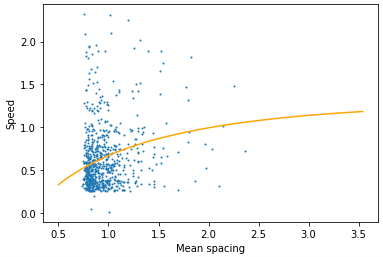
\includegraphics[scale=0.85]{images/vadere-bottleneck-obs.png}}
    \hfill
    \subfloat[b]{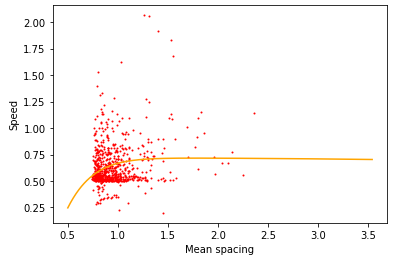
\includegraphics[scale=0.85]{images/vadere-bottleneck-nn.png}}
    \caption{\textbf{Bottleneck: }FD model trained on observations (a) and FD model trained on NN predictions (b)}
    \label{fig:vadere-bottleneck-result}
\end{figure}

Before closing up the task we went for a more semantically interpretable result. In particular we created two FD models regarding the previously discussed \textit{corridor} scenario. The first model is fitted on the observation data, giving physical meaning to the dynamical system with the \textit{desired speed}, \textit{pedestrian size} and \textit{time gap} parameters. The second model is fitted instead on the prediction data (created thanks to the fitted NN), giving analogous meaning to the generated samples. 

The result is successful if the parameters of the fitting on observations is comparable to the fitting on predictions. In \textbf{\hyperref[fig:vadere-fd-comp-visual]{Figure \ref{fig:vadere-fd-comp-visual}}} one can appreciate the FD fitted on the observations (which are in \textit{blue}) vs the FD fitted on the predictions (which are in \textit{red}).

\begin{figure}[H]
    \centering
    \subfloat[a]{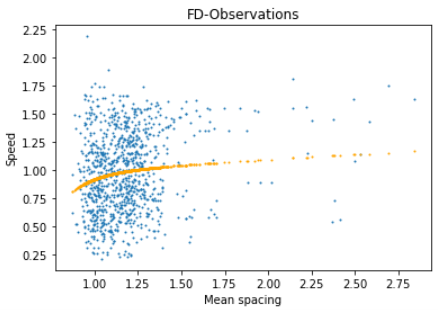
\includegraphics[scale=0.85]{images/vadere-obs-sub.png}}
    \hfill
    \subfloat[b]{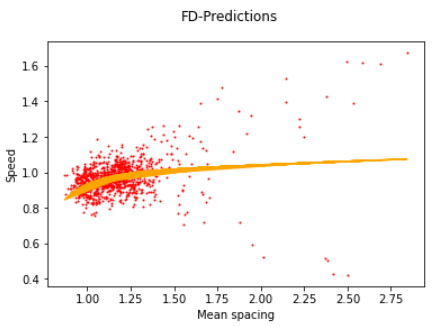
\includegraphics[scale=0.85]{images/vadere-pred-sub.png}}
    \caption{Observations and FD fitted (a) Predictions and FD fitted (b)}
    \label{fig:vadere-fd-comp-visual}
\end{figure}

What is immediately noticeable is that the predictions have a different \textit{shape} with respect to the observations, leading to thinking the network has failed to approximate the data. The result is in fact fundamentally different from the already shown \textbf{\hyperref[fig:vadere-corridor-result]{Figure \ref{fig:vadere-corridor-result}}}. But since the MSE result was good we continued the experiment nevertheless, trying to understand which are the parametric values of the two generated FD models.

Since the parameters should be non other than the values coming out of the three nodes in the FD network output layer (by construction), we decided to save the batch average of these output values in a convenience structure (simple dictionary) while training. This means that for each batch of training we save the average value of each of the output nodes in a dictionary, creating therefore three indexed lists with the same length of the number of training batches. 

The line of thought is that we expect the parameters to more or less stabilize toward a value the more the training goes on. This effect fortunately happened and is visible in \textbf{\hyperref[fig:vadere-fd-params-batch]{Figure \ref{fig:vadere-fd-params-batch}}}, showing the stabilization as the training advances. 

\begin{figure}[h]
    \centering
    \subfloat[a]{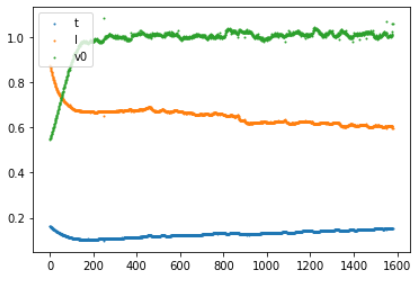
\includegraphics[scale=0.85]{images/vadere-fd-params-obs.png}}
    \hfill
    \subfloat[b]{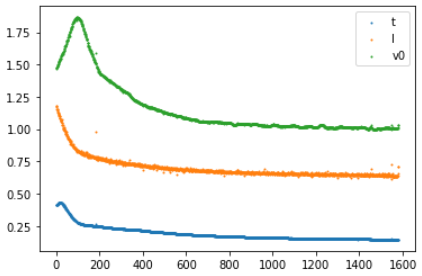
\includegraphics[scale=0.85]{images/vadere-fd-params-pred.png}}
    \caption{Parameters values batch by batch, showing stabilization}
    \label{fig:vadere-fd-params-batch}
\end{figure}

Therefore we took empirically the last thousand iterations as the stabilized values for the parameters and we defined as final parameters of the FD model the average of these iterations. The results are shown in \textbf{\hyperref[tab:vadere-fd-comparison]{Table \ref{tab:vadere-fd-comparison}}}. It is at this point clear that the network has indeed generated predictions which give the same physical meaning as the observations, as the two FD models have extremely close parametric values.

\begin{table}[H]
    \centering
    \begin{tabular}{|ccc|}
        \hline
        \textbf{Parameter} & \textbf{FD on obs} & \textbf{FD on pred}\\
        \hline
        \hline
        \textit{desired speed} & 1.013 & 1.015\\
        \hline
        \textit{pedestrian size} & 0.616 & 0.649\\
        \hline
        \textit{time gap} & 0.142 & 0.15\\
        \hline
    \end{tabular}
    \caption{Parameter comparison between FD fitted on observations vs on predictions}
    \label{tab:vadere-fd-comparison}
\end{table}

\end{task}


\begin{task}{4, Comparison to the paper's results}
Objective of this task is to try and reproduce the paper's results, which are fundamentally achieved sequentially:
\begin{itemize}
    \item Firstly, the researchers take into consideration a scenario (which one? Do not ask, there are things which humans are not worthy of knowing yet) and train models with incrementally big architectures on it. They utilize \textit{sigmoid} as activation function and show how the incredibly small architecture with \texttt{(3,)} is the best performing (\textbf{\hyperref[fig:nn-training-curves]{Figure \ref{fig:nn-training-curves}}}). 
    \item Secondly, after fixing the best architecture, they take a scenario for \textit{corridor} and a scenario for \textit{bottleneck} into consideration, training and testing multiple models on different combinations of training/testing scenario. \textbf{\hyperref[fig:nn-vs-fd]{Figure \ref{fig:nn-vs-fd}}} shows how the NN gets increasingly better performances with respect to the FD model, especially when being trained on mixed scenarios, showing how the model is capable of distinguishing better the situations.
    \item Last result to reproduce is more on the semantics of the NN results. The researchers fit an FD on the NN predictions to show that the \textit{meaning} of the NN fitting goes to recreate data with approximately the same modelled \textit{desired speed}, \textit{pedestrian size} and \textit{time gap}. Paper result comparison are shown in \textbf{\hyperref[fig:fd-parameters]{Figure \ref{fig:fd-parameters}}}
\end{itemize}
\begin{figure}[h]
    \centering
    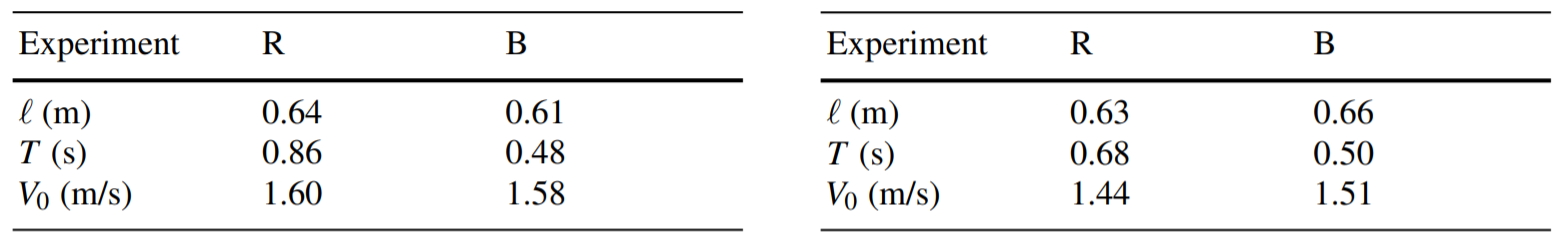
\includegraphics[scale=0.5]{images/fd_parameters.png}
    \caption{FD parameters of model fitted on observations (\textit{left}) vs fitted on predictions (\textit{right}).}
    \label{fig:fd-parameters}
\end{figure}

\paragraph{Results on different scenarios}
We trained the network on various scenarios: bottlenecks of 70 and 120 centimeters  and corridors with 85 and 140 pedestrians.
We used a bootstrap with 5 subsamples of 5000 elements performing a 5-fold cross validation (time constraints and available computation power reduced the number of bootstraps we could unfortunately try).
The learning curves are reported in Figure \ref{fig:various-scenarios}.
As we can see, the results in terms of MSE are comparable to the ones in the paper, sometimes even better.
Furthermore, the learning curves tend to be pretty different depending on the scenario, this probably means that the plot of the paper refers to a specific scenario, and so obtaining the exact same curve is not that important.
The network with one hidden layer with three units tends to provide good results, but it is curious how in the case of the bottleneck of 70 centimeters, the best model has one hidden layer, but two units.
Moreover, in the case of the corridor of 140 centimeters, the network denoted by (10, 4) has comparable performance to (3,), but the latter is simpler and thus preferable.
Nevertheless, from (5, 2) on the testing loss is starting to decrease significantly, suggesting that bigger models might actually surpass (3,) on that scenario.

\begin{figure}[h]
    \centering
    \subfloats[a]{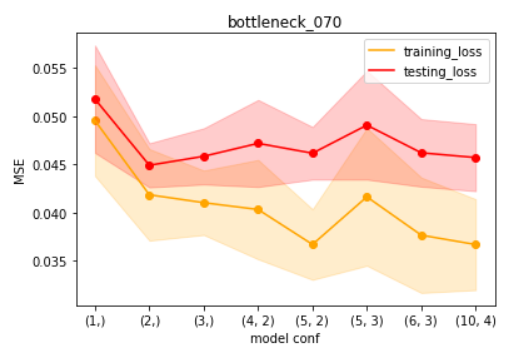
\includegraphics[width=0.45\textwidth]{images/bottleneck_70.png}}
    \hfill
    \subfloats[b]{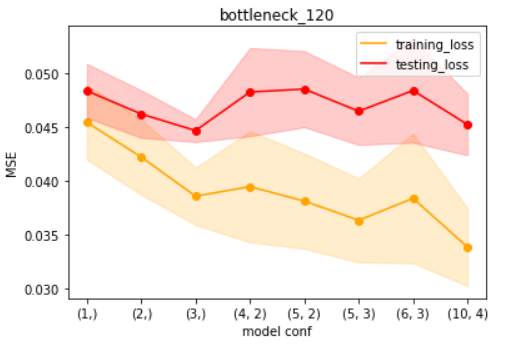
\includegraphics[width=0.45\textwidth]{images/bottleneck_120.png}}\\
    \subfloats[c]{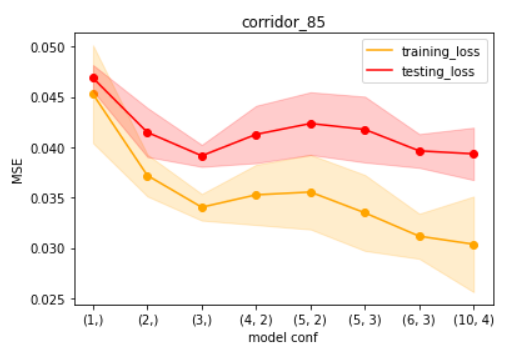
\includegraphics[width=0.45\textwidth]{images/corridor_85.png}}
    \hfill
    \subfloats[d]{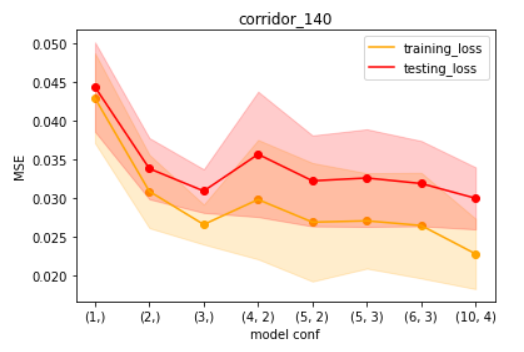
\includegraphics[width=0.45\textwidth]{images/corridor_140.png}}
    \caption{Learning curves of different networks achitectures on different scenarios.}
    \label{fig:various-scenarios}
\end{figure}

\paragraph{Results on different combos of Corridor and Bottleneck}
To obtain this results we fixed the architecture to the one utilized in the paper: \texttt{(3,)}. We therefore went through the results we got in the previous paragraph, and eventually selected the two scenarios \textit{Bottleneck\_120} and \textit{Corridor\_85} to create the needed combinations, as they performed best with that architecture. Each result present in \textbf{\hyperref[fig:fdvsnn]{Figure \ref{fig:fdvsnn}}} was created by training the FD model using bootstrapping and cross validation (5 subsamples of 5000 samples each, 5 fold cv, early stopping) and training the NN to create the predictions, training in the same way. Testing of both models was done on the selected testing set (e.g. for B/C we trained models on the bottleneck scenario and tested them on the corridor) and the resulting MSEs created what can be seen in the figure.

It is clear that the results are differing from \textbf{\hyperref[fig:nn-vs-fd]{Figure \ref{fig:nn-vs-fd}}}. In our results the NN model performs better than the FD model in all cases but the most peculiar ones, having the testing data fundamentally different from the training one. Although the NN model performs better in almost all cases, it does not \textit{greatly} outperform the FD model and also the MSEs look much higher for both of the models, when compared to the paper's results. To be honest this was not the result we expected and even trying different combinations of scenarios (e.g. we tried to produce the figure with all the combinations between \textit{Bottleneck\_120}, \textit{Bottleneck\_180}, \textit{Corridor\_85} and \textit{Corridor\_140}) did not give results that were fundamentally different from the ones proposed. After various testings, time constraints stopped us from further investigating the motivations for these differences. What we suspect is again a difference in method between us and the researchers. As already seen in the last paragraph, as it highlighted some differences in results, the same could possibly have happened here.

\begin{figure}[h]
    \centering
    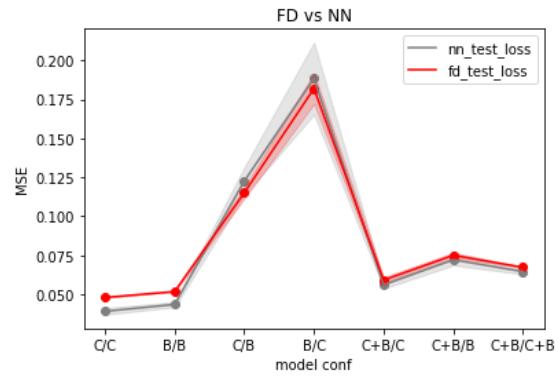
\includegraphics[scale=0.85]{images/fdvsnn.png}
    \caption{Comparison of test losses on models constructed with different train/test combos.}
    \label{fig:fdvsnn}
\end{figure}

\paragraph{NN meaning through FD parameters}
We continued our comparison towards a more interpretable result, trying to replicate the third result of the paper (\textbf{\hyperref[fig:fd-parameters]{Figure \ref{fig:fd-parameters}}}). To do so we first set a couple of scenarios, in this case \textit{Corridor\_85} and \textit{Bottleneck\_070}. The main objective here is to construct two different FD Weidmann models per each scenario through the training already proposed in \textbf{Task 2} and compare the results between the two (again per each scenario), in a similar fashion to what we already achieved at the end of \textbf{Task 3}. The main difference is that this time we are working with not self-constructed data.

During the implementation we faced an obstacle we had already faced for the same goal in \textbf{Task 3}, regarding the gathering of output values from the three output nodes. Since we train the net by an MSE loss constructed between the output ground truth speed and the Weidmann formula created by the three output nodes, we do not actually get in output the nodes values, but only the predicted speed. So, to store the nodes outputs we need to update the aforementioned dictionary (explained in \textbf{Task 3}) inside the model \texttt{call} method, leading to the need of an \textit\textbf{eagerly run}. Abilitating the \textbf{eagerly run} considerably slows down the execution, a problem which was not that relevant in the Vadere datasets since they are relatively little (less than 2000 samples), but absolutely time consuming in the bigger datasets used by the paper. All of this to say that we had eventually to take a random subsample of the datasets (we decided to make the subsample with dimension 10000) to fit the delivery time constraints.

Eventually we built the two models for each one of the considered scenarios, as can be seen in \textbf{\hyperref[fig:various-fd-comparison]{Figure \ref{fig:various-fd-comparison}}}, where first row compares corridor scenario (FD model on observables (left) and predictions (right)) and second row goes instead for the bottleneck scenario. 

\begin{figure}[h]
    \centering
    \subfloats[a]{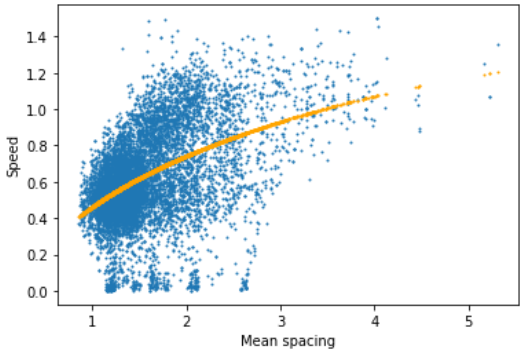
\includegraphics[width=0.45\textwidth]{images/res-corr-obs-fd.png}}
    \hfill
    \subfloats[b]{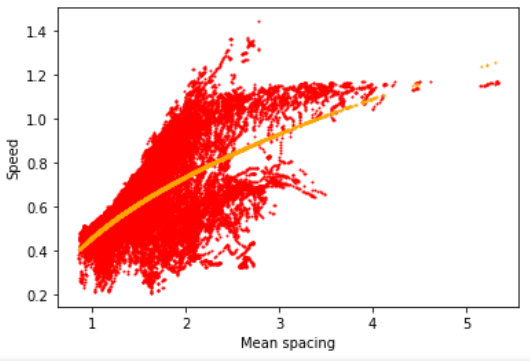
\includegraphics[width=0.45\textwidth]{images/res-corr-pred-fd.png}}\\
    \subfloats[c]{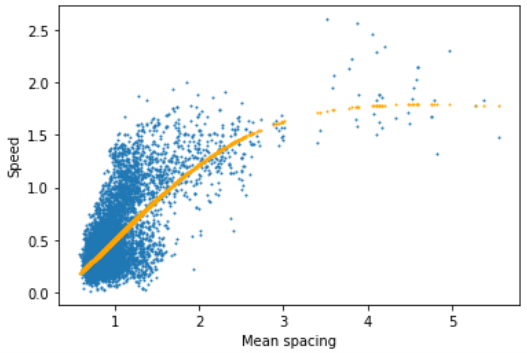
\includegraphics[width=0.45\textwidth]{images/res-bott-obs-fd.png}}
    \hfill
    \subfloats[d]{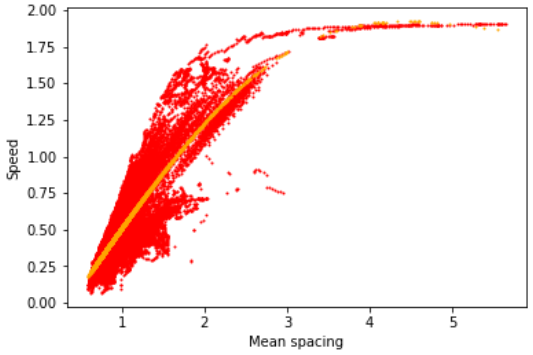
\includegraphics[width=0.45\textwidth]{images/res-bot-pred-fd.png}}
    \caption{Data observable (\textit{left}) and predictions(\textit{right}) with respective FD model. Both Bottleneck\_070 (\textit{bottom}) and Corridor\_85 (\textit{top}).}
    \label{fig:various-fd-comparison}
\end{figure}

As we mentioned already at the end of \textbf{Task 3}, from these training we got the parameters value batch by batch, as average of the output nodes per single batch. Plotting these values should show some reaching of stability, and that actually happens as shown in \textbf{\hyperref[fig:various-fd-parameters]{Figure \ref{fig:various-fd-parameters}}}.

\begin{figure}[h]
    \centering
    \subfloats[a]{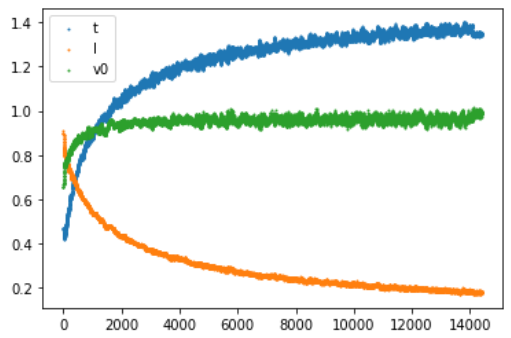
\includegraphics[width=0.45\textwidth]{images/res-corr-obs-par.png}}
    \hfill
    \subfloats[b]{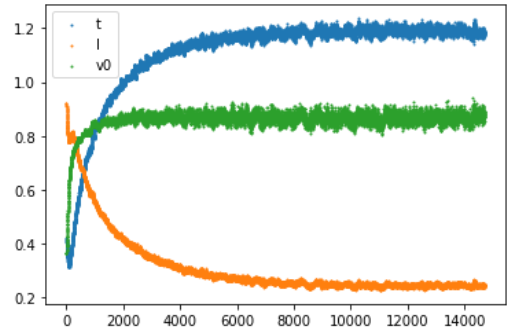
\includegraphics[width=0.45\textwidth]{images/res-corr-pred-par.png}}\\
    \subfloats[c]{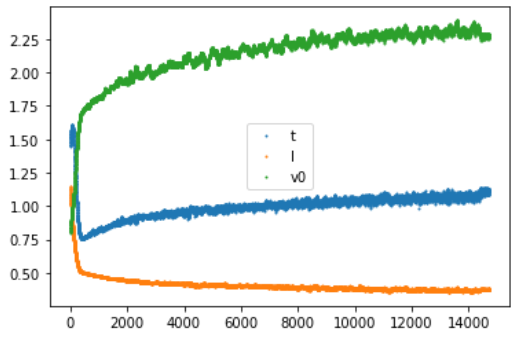
\includegraphics[width=0.45\textwidth]{images/res-bot-obs-par.png}}
    \hfill
    \subfloats[d]{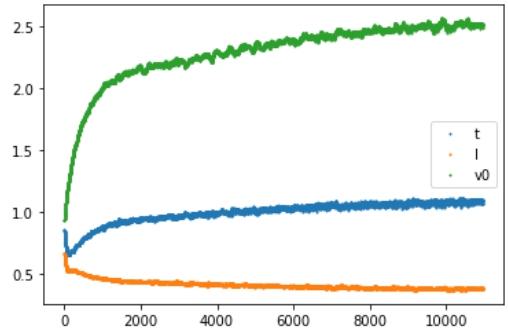
\includegraphics[width=0.45\textwidth]{images/res-bot-pred-par.png}}
    \caption{Parameters stabilization: FD model on corridor observable (\textit{top left}), corridor prediction (\textit{top right}), bottleneck observables (\textit{bottom left}) and bottleneck predictions (\textit{bottom right}).}
    \label{fig:various-fd-parameters}
\end{figure}

Again from these plots we empirically chose to cut the end of these zigzags, getting the final ensemble of parameter values to formulate and identify the definitive parameter values as averages of these ensembles. The comparison between the FD models on observables and predicted are shown in \textbf{\hyperref[tab:res-fd-comparison]{Table \ref{tab:res-fd-comparison}}}, highlighting how the physical meaning of the generated data is catching the real meaning of the observables even though the predictions differ in shape with said observables.

\begin{table}[H]
    \centering
    \begin{tabular}{|cccc|}
        \hline
        \textbf{\textit{model}} & \textbf{\textit{desired speed}} & \textbf{\textit{pedestrian size}} & \textbf{\textit{time gap}}\\
        \hline
        \hline
        \textit{FD Corridor Observations} & 0.957 & 0.274 & 1.259\\
        \hline
        \textit{FD Corridor Predictions} & 0.867 & 0.287 & 1.146\\
        \hline
        \hline
        \textit{FD Bottleneck Observables} & 2.176 & 0.399 & 1.004\\
        \hline
        \textit{FD Bottleneck Predictions} & 2.354 & 0.404 & 1.019\\
        \hline
    \end{tabular}
    \caption{Parameter comparison between FD fitted on observations vs on predictions}
    \label{tab:res-fd-comparison}
\end{table}

\paragraph{Dropout}
Since in the paper the best model was very simple - one hidden layer with three units - and bigger models were leading to overfitting, we though that it might be a good idea to add regularization to tackle this phenomenon without reducing too much the complexity of the network.
We tested both geometries, respectively the bottleneck of 70cm and the corridor of 85cm.
In both cases we applied dropout after each fully-connected ("Dense" in Tensorflow) layer, with value 0.3 and 0.1.
Unfortunately the results are not very good and Figure \ref{fig:dropout} shows that probably this technique was too harsh and led to the opposite effect, i.e. a sort of underfitting.

\begin{figure}[H]
    \centering
    \subfloats[a]{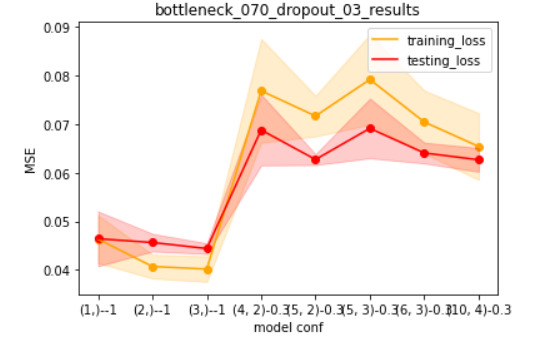
\includegraphics[width=0.45\textwidth]{images/dropout1.png}}
    \hfill
    \subfloats[b]{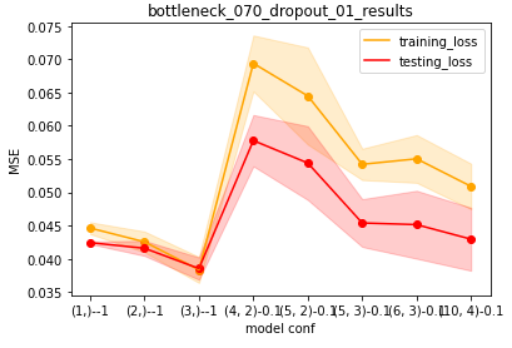
\includegraphics[width=0.45\textwidth]{images/dropout3.png}}\\
    \subfloats[c]{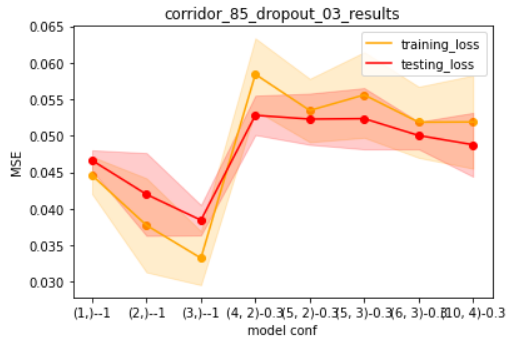
\includegraphics[width=0.45\textwidth]{images/dropout2.png}}
    \hfill
    \subfloats[d]{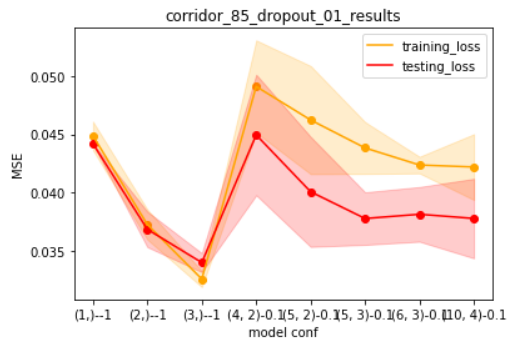
\includegraphics[width=0.45\textwidth]{images/dropout4.png}}
    \caption{Results with dropout.
    The first row report the results on the bottleneck scenario with 70 pedestrians, while the second one is for the corridor scenario with 85 pedestrians.
    The plots in the first column have a dropout of 0.3, while in the second column the droout value is 0.1.}
    \label{fig:dropout}
\end{figure}

\paragraph{Principal components analysis}
We performed some experiments increasing or decreasing the number of attributes in the data used to train the neural network, trying to understand if the approach of the paper was improvable from this point of view.
A natural development of this was to try to apply the PCA to the data and train the network in the PCA space, using a certain number of principal components.
We tested the configurations and obtained the data reported in Table \ref{tab:pca}

\begin{table}[h]
    \centering
    \begin{tabular}{|c|c|c|}
        \hline
        \textbf{Energy retained} & \textbf{Number of principal components} & \textbf{Loss}\\
        \hline
        100\% & 21 & 0.03748 (std dev: 0.0013)\\
        91.04\% & 17 &  0.03916 (std dev: 0.0019)\\
        75.12\% & 12 &  0.03939 (std dev: 0.0006)\\
        54.59\% & 7 &  0.04121 (std dev: 0.0013)\\
        23.03\% & 2 &  0.05911 (std dev: 0.0005)\\
        \hline
    \end{tabular}
    \caption{Configuration and results obtained using PCA on the data to train the network.}
    \label{tab:pca}
\end{table}

As we can see, 12 principal components provide anyway a good approximation with almost half of the inputs size.
With 7, results start getting worse, bust still not that terrible, while with 2 - as can be expected - the loss increases and it is significantly worse than the one of equivalent models trained with the original data.
Overall we think this is a nice way to reduce the input size, improving the speed of training, without manually selecting actual attributes to remove, leading probably to much worse performance.

\paragraph{Reduced input size}
The input of the neural network consists of 21 attributes: the mean spacing of the pedestrian w.r.t. its 10 nearest neighbors and the relative positions of those neighbors expressed as couples of coordinates $x-x_i$ and $y-y_i$.
The mean spacing, therefore, can be derived from those neighbors positions.
For this reason, we wanted to check if this attribute is really important and we tried to train and test a NN with the same data used so far, but without the mean spacing.
The results are depicted in Figure \ref{fig:no-mean-spacing}, where the scenarios bottleneck with 70 people and corridor with 85 were used to test different architectures of neural networks (reported in the x-axis of each plot in Fig. \ref{fig:no-mean-spacing}).
As it is possible to see, compared to the case with the original data (1st columns of Fig. \ref{fig:no-mean-spacing}), removing the mean spacing actually degrades slightly the performance (2nd column of Fig. \ref{fig:no-mean-spacing}).
We can conclude that the attribute in object could be removed, with a small penalty in MSE.
The obtained speedup, though, is negligible, therefore it might be wiser to instead keep it in the data.
It would be interesting to experiments with a smaller number of nearest neighbors, but we were not able to do that due to time constraints.

\begin{figure}[h]
    \centering
    \subfloats[a]{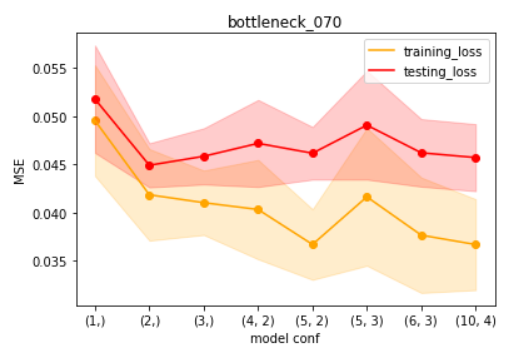
\includegraphics[width=0.45\textwidth]{images/bottleneck_70.png}}
    \hfill
    \subfloats[b]{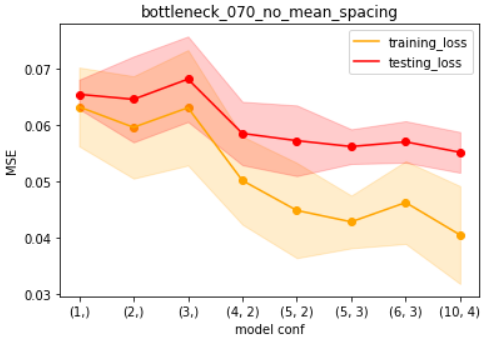
\includegraphics[width=0.45\textwidth]{images/bottleneck_70_no_mean_spacing.png}}\\
    \subfloats[c]{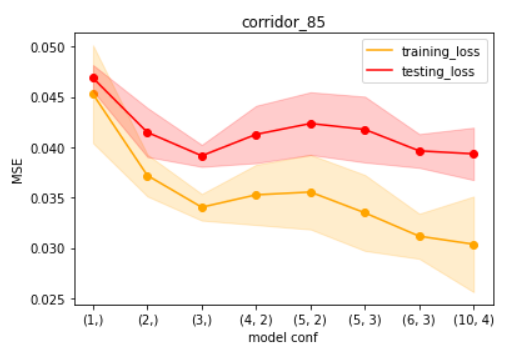
\includegraphics[width=0.45\textwidth]{images/corridor_85.png}}
    \hfill
    \subfloats[d]{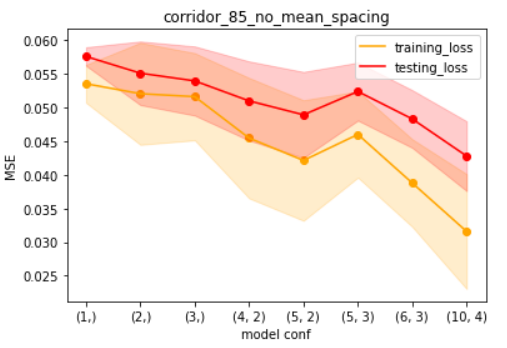
\includegraphics[width=0.45\textwidth]{images/corridor_85_no_mean_spacing.png}}
    \caption{Comparison of the same networks trained with (1st columns) and without (2nd columns) mean spacing.}
    \label{fig:no-mean-spacing}
\end{figure}

\paragraph{Change activation function}
On a side note, we also attempted changing the hidden layer activation function from \textit{sigmoid} to \textit{tanh}. We did not attempt \textit{relu} since it is an activation function introduced for reasons connected to gradient propagation problem in much deeper nets, which is not our case at all. The results came out quite similar to the use of \textit{sigmoid} and for sure not noteworthy even when changing the scenario at hand. 
\end{task}


\begin{task}{5, Discussion on the approach and architecture}
The classic approach to predict pedestrians' behavior is the fundamental diagram, which infers for example the speed as a function of few parameters with a clear physical meaning (e.g. mean spacing, time gap, etc.).
This approach can be unsatisfactory in case of complex geometries, which of course influence the pedestrians' dynamics.
For this reason, Tordeux et al. \cite{tordeux2018} propose to use a different approach: use a neural network, which instead has many parameters, but none of them has a clear meaning.
The authors show how this model actually performs better, especially in cases of mixed scenarios (Figure \ref{fig:nn-vs-fd}) and that it is able to tell apart different geometries, in fact, when fitting the FD model on the NN's predictions, two distinct curves appear, one for the bottleneck and one for the corridor (Figure \ref{fig:fd-curves-fitted-nn-preds}), highlighting that the network's prediction for one geometry and the other lie on two different distributions.\\
However, we noticed that different scenarios were producing substantially different plots and results, but in the paper only one specific scenario looks to be used, without actually specifying which one it is or how they got that specific ensemble of data.
They also say that the pedestrians' speeds are given, but they actually need to be derived from the positions and the frame rate, since they are not present in the dataset.
Even though computing them is pretty straight forward, there might be some details in the authors' process that a reader might miss.
More in general, a lot of information is missing in the paper, making it difficult for the readers to exactly reproduce those results.
For example, they state that the training is performed through bootstrapping, but the size of the different subsamples and the number of folds in the cross-validation are not specified.
The same happens for almost all the training hyperparameters such as the batch size, the number of epochs, the learning rate and so on.
The best model is the neural network with only 3 hidden units, which is peculiar, being unusually shallow and simple.
At this point they might have tried to apply some regularization techniques on larger networks, but this was not tested.
Furthermore, as we have shown previously, some larger networks actually perform similarly to the one with 3 hidden neurons, and the error is in a descending trend as the complexity of the models increases (after a local minimum at (3,)).
This further encourages to try larger networks with regularization as they might actually outperform simpler models.
Our results with dropout were not better than the ones without it, but a more extensive test could be carried on, also with different regularization techniques other than dropout.\\
As a final point, we would like to mentions few additions and extensions that could be made to the project.
First of all, our results using PCA seem promising, it could be exploited and other dimensionality reduction techniques could be explored.
We also noticed that removing mean spacing degrades the performance a bit, but what about changing the number of nearest neighbors to be considered?
Furthermore, our dropout was probably too harsh, but it could be tested on more complex geometries such as T-junctions, supermarkets simulations etc., which might require more complex networks where regularization is needed.
Also, since we have information about the time (i.e. the time steps), it would be interesting to exploit it taking into consideration the speed of the pedestrian in the previous time step, using models such as RNNs or HMMs, encoding information about the past to predict the speed at each time step, while so far the time information was simply lost, sending to the network some "screenshots" of the simulation in a random order.
One last, more ambitious attempt could be to use imitation learning / reinforcement learning to learn an agent who behaves like a pedestrian and learns to interact with others (avoiding them and dynamically changing its speed).
The observations could be considered as expert's trajectories and, after having such agent, many of them could be placed in a scenario with a desired geometry to simulate the behavior of a crowd, making it possible for us to simply "read" their speeds.
\end{task}

\newpage
\bibliographystyle{plain}
\bibliography{Literature}

\end{document}